\documentclass{article}
\usepackage{amsmath, amssymb, amssymb}
\usepackage{tikz}

\begin{document}
\begin{center}
    \begin{LARGE}
        \textbf{Introduction to Electromagnetism}
    \end{LARGE}
\end{center}

\section{Coulomb's Law}

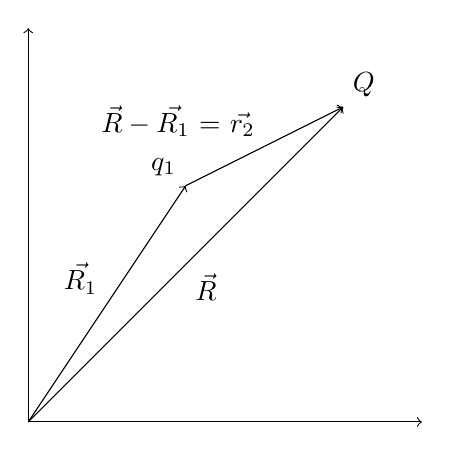
\begin{tikzpicture}
    \draw[->] [black] (0,0) -- (0, 5);
    \draw[->] [black] (0,0) -- (5, 0);
    \draw[black] (0,0) -- (2,2) node[anchor=north west] {$\vec{R}$};
    \draw[->] [black] (2,2) -- (4,4) node[anchor=south west] {$Q$};
    \draw[black] (0, 0) -- (1,1.5) node[anchor=south east] {$\vec{R_1}$};
    \draw[black, ->] (1,1.5) -- (2,3) node[anchor=south east] {$q_1$};
    \draw[black] (2,3) -- (3,3.5) node[anchor=south east] {$\vec{R} - \vec{R_1}$ = $\vec{r_2}$};
    \draw[->] [black] (3,3.5) -- (4,4);

\end{tikzpicture}

the force on $Q$ due to $q_1$ is given by:
$$\vec{F_1} = \frac{1}{4\pi\epsilon_0} \frac{q_1Q}{r_1^2} \hat{r_1}$$

If there was another charge $q_2$ at $\vec{r_2}$: 

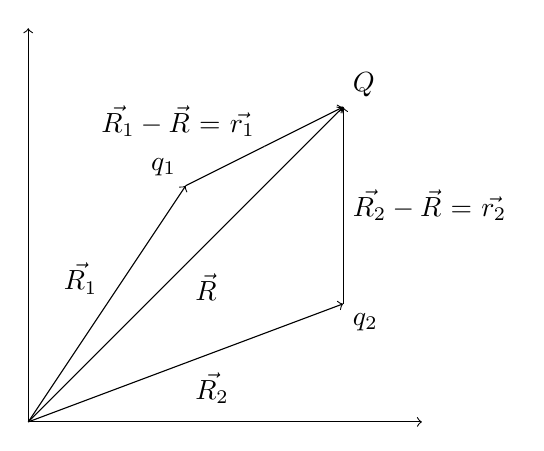
\begin{tikzpicture}
    \draw[->] [black] (0,0) -- (0, 5);
    \draw[->] [black] (0,0) -- (5, 0);
    \draw[black] (0,0) -- (2,2) node[anchor=north west] {$\vec{R}$};
    \draw[->] [black] (2,2) -- (4,4) node[anchor=south west] {$Q$};
    \draw[black] (0, 0) -- (1,1.5) node[anchor=south east] {$\vec{R_1}$};
    \draw[black, ->] (1,1.5) -- (2,3) node[anchor=south east] {$q_1$};
    \draw[black] (2,3) -- (3,3.5) node[anchor=south east] {$\vec{R_1} - \vec{R}$ = $\vec{r_1}$};
    \draw[->] [black] (3,3.5) -- (4,4);
    \draw[black] (0, 0) -- (2,0.75) node[anchor=north west] {$\vec{R_2}$};
    \draw[black, ->] (2,0.75) -- (4,1.5) node[anchor=north west] {$q_2$};
    \draw[black] (4,1.5) -- (4,2.75) node[anchor=west] {$\vec{R_2} - \vec{R}$ = $\vec{r_2}$};
    \draw[->] [black] (4,2.75) -- (4,4);

\end{tikzpicture}

The force on $Q$ due to $q_2$ is given by:
$$\vec{F_2} = \frac{1}{4\pi\epsilon_0} \frac{q_2Q}{r_2^2} \hat{r_2}$$

And the net charge on $Q$ is given by:
$$\vec{F} = \vec{F_1} + \vec{F_2}$$
$$\vec{F} = \frac{1}{4\pi\epsilon_0} \frac{q_1Q}{r_1^2} \hat{r_1} + \frac{1}{4\pi\epsilon_0} \frac{q_2Q}{r_2^2} \hat{r_2}$$

If there were $n$ charges, the net force on $Q$ would be:
$$\vec{F} = \sum_{i=1}^n \frac{1}{4\pi\epsilon_0} \frac{q_iQ}{r_i^2} \hat{r_i}$$
$$\vec{F} = Q \sum_{i=1}^n \frac{1}{4\pi\epsilon_0} \frac{q_i}{r_i^2} \hat{r_i}$$

where $\sum_{i=1}^n \frac{1}{4\pi\epsilon_0} \frac{q_i}{r_i^2} \hat{r_i}$ is the electric field $\vec{E}$ at $\vec{R}$ due to the $n$ charges.

\textbf{Field}: A value, vector or tensor, that is defined for every point in space and time.\\[1pt] 

\section{Vector Calculus}


\end{document}